% Template: LaTeX file for ICMC 2010 papers, with hyper-references
%
% derived from the DAFx-06 templates
% derived from the ICMC 2009 templates by Steve Beck
%
% 1) Please compile using latex or pdflatex.
% 2) Please use figures in vectorial format (.pdf); .png or .jpg are working otherwise 
% 3) Please use the "papertitle" and "pdfauthor" commands defined below

%------------------------------------------------------------------------------------------
\documentclass[twoside,10pt]{article}
\usepackage{icmc2010,amssymb,amsmath} 
%\setcounter{page}{1}

\usepackage{mathptmx} 

%____________________________________________________________
%  !  !  !  !  !  !  !  !  !  !  !  ! user defined variables  !  !  !  !  !  !  !  !  !  !  !  !  !  !
%==== set the title ====
\def\papertitle{Paper Template for ICMC 2010, Stony Brook University, NY}
%\def\papertitle{}	%-- should be empty for the submission anyway!

%==== 1st submission: author name and affiliation are empty for anonymous submission ====
\def\paperauthorA{} 
\affiliation{}{}


%==== final submission: author name and affiliation ====
%---- uncomment 1 to 4 lines, for 1 to 4 authors
\def\paperauthorA{First Author}
\def\paperauthorB{Second Author}
\def\paperauthorC{Third Author}
\def\paperauthorD{Fourth Author}

%%---- set correspnding affiliation data for...
%%-- 1 author
%\affiliation{\paperauthorA}
%  {School\\ Department, City, Country \\ {\tt \href{mailto:email@domain.icmc}{email@domain.icmc}}}

%%-- 2 authors with same affiliation
%\affiliation{\paperauthorA, \paperauthorB}
%  {School\\ Department, City, Country \\ {\tt \href{mailto:email@domain.icmc}{email@domain.icmc}}}

%-- 2 authors with different affiliations
%\twoaffiliations{\paperauthorA}{School\\ Department}
%  {\paperauthorB}{Company\\ Address}

%%-- 3 authors with different affiliations
%\threeaffiliations{\paperauthorA}{School A\\ Department X}
%  {\paperauthorB}{Company\\ Address}
%  {\paperauthorC}{School B\\ Department Y}

%%-- 4 authors with different affiliations
%\fouraffiliations{\paperauthorA}{School A\\ Department X}
%  {\paperauthorB}{Company\\ Address}
%  {\paperauthorC}{School B\\ Department Y}
%  {\paperauthorD}{School C\\ Department Z}

%  ^  ^  ^  ^  ^  ^  ^  ^  ^  ^ user defined variables  ^  ^  ^  ^  ^  ^  ^  ^  ^  ^  ^  ^ 
%------------------------------------------------------------------------------------------

%%-- if using .ps or .eps figure files, they will be converted on the fly
%%-- RMK: for faster LaTeX runs, use it only once after adding new \includegraphics[]{} cmds
%\usepackage{epstopdf}	 

%---- the hyperref package must be last to properly work
\usepackage[pdftex,
       pdftitle={\papertitle},
	pdfauthor={\paperauthorA},
	colorlinks=false,bookmarksnumbered,pdfstartview=XYZ]{hyperref}
%\pdfcompresslevel=9
\usepackage[pdftex]{graphicx}	% for compatible graphics with hyperref
\usepackage[figure,table]{hypcap}	% corrects the hyper-anchor of figures/tables

\title{\papertitle}

%------------------------------------------------------------------------------------------
\begin{document}

\DeclareGraphicsExtensions{.png,.jpg,.pdf} % used graphic file format for pdflatex
    
\maketitle



\begin{abstract}

This paper presents an object-oriented, reflective, application programming interface for C++, with an emphasis on real-time signal processing. It makes use of polymorphic typing, dynamic binding, and introspection to create a cross-platform environment pulling ideas from languages such as Smalltalk and Objective-C while remaining within the bounds of the portable and cross-platform C++ context.  The Jamoma Foundation and DSP Library provide a flexible framework and runtime environment, as well as an expanding collection of unit generators for synthesis, processing, and analysis.  This library has been used in both open source and commercial software projects over the past seven years including Electrotap's Tap.Tools, Cycling '74's Hipno, and the Jamoma Modular Framework.

\end{abstract}



\section{Introduction}\label{sec:introduction}

This template includes all the information about formatting manuscripts
for the ICMC 2010. Please follow these guidelines to give the final
proceedings a uniform look. 

\section{Page Size}\label{sec:page_size}

The proceedings will be printed on US letter paper (8.5" $\times$ 11", or 21.6~cm $\times$ 28~cm). 
All material on each page should fit within a rectangle of 6.9" $\times$ 9" (17.5~cm $\times$ 22.9~cm), centered on the page, beginning 1" (2.5~cm) from the top of the page and ending 1" (2.5~cm) from the bottom.  
The left and right margins should be 0.8" (2~cm).
The text should be in two 3.3" (8.4~cm) columns with a 0.3" (0.8~cm) gutter. All {\it text} must be in a two-column format. Text must be fully justified.


\section{Typeset text}\label{sec:typeset_text}

\subsection{Normal or Body Text}\label{subsec:body}

Please use a 10pt (point) Times font, or other Roman font with serifs, as close as possible in appearance to Times. Please use sans-serif or non-proportional fonts only for special purposes, such as distinguishing source code text.

The first paragraph in each section should not be indented, but all other paragraphs should be.

\subsection{Title and Authors}

The title is 14pt Times, bold, caps, upper case, centered. Authors' names are centered. The lead author's name is to be listed first (left-most), and the co-authors' names after. If the addresses for all authors are the same, include the address only once, centered. If the authors have different addresses, put the addresses, evenly spaced, under each authors' name.

\subsection{Page Numbering, Headers and Footers}

Do not include headers, footers or page numbers in your submission. These will be added when the publications are assembled.

\section{First level headings}

First level headings are in Times 10pt bold, centered with 12 pt of space above the section head, and 12 pt space below it.  For a section header immediately followed by a subsection header, the space should be merged to 12 pt total.

\subsection{Second Level Headings}

Second level headings are in Times 10pt bold, flush left, with 12 pt of space above the section head, and 6 pt space below it.  The first letters of significant words are capitalized.

\subsubsection{Third level headings}

Third level headings are in Times 10pt italic, flush left, with 12 pt line of space above and 6 pt space below the section head. More than three levels are highly discouraged.  The first word is capitalized.

\section{Footnotes and Figures}

\subsection{Footnotes}

Indicate footnotes with a number in the text\footnote{This is a footnote.}.
Use 8pt type for footnotes. Place the footnotes at the bottom of the page
on which they appear. Precede the footnote with a 0.5pt horizontal rule.

\subsection{Figures, Tables and Captions}

All artwork must be centered, neat, clean, and legible. All lines
should be very dark for purposes of reproduction and art work should
not be hand-drawn.  The proceedings is not in color and therefore all
figures must make sense in black-and-white form.  Figure and table
captions, with numbers, always appear below the figure. Leave 1 line
space between the figure or table and the caption. Each figure or
table is numbered consecutively. Captions should be Times 10pt.

\begin{table}[htbp]
\begin{center}
\begin{tabular}{|l|l|}
\hline
String value & Numeric value \\
\hline
hello ICMC  & 1073 \\
\hline
\end{tabular}
\end{center}
\caption{Table captions are placed below the table.}
\label{tab:example}
\end{table}

\begin{figure}[htbp]
\centerline{\framebox{
	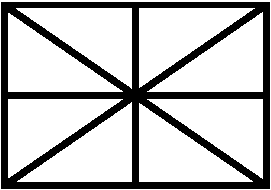
\includegraphics[width=0.9\columnwidth]{figure}}}
\caption{Figure captions are placed below the figure.}
\label{fig:example}
\end{figure}
Place tables/figures in text as close to the reference as possible
(see Figure~\ref{fig:example} and Table~\ref{tab:example}). They may extend
across both columns to a maximum width of 17.5cm (6.9").

\section{Equations}

Equations should be placed on separated lines and numbered.
The number should be on the right side.

\begin{equation}
E=mc^{2}
\end{equation}

\section{Citations}

All bibliographical references should be listed at the
end, inside a section named ``REFERENCES'', numbered
and in alphabetic order. Also, all
references listed should be cited in the text.
To do so, use the \texttt{IEEEtranS.bst} bibliography 
style (as it will automatically sort your reference), and 
collect the full bibliography information in a separate 
file (e.g. \texttt{template.bib} in the case of these 
templates).
To refer to a document, use the \verb+\cite{}+ command 
to make it appear in square brackets \cite{Someone:02,Author:00}.

\section{Filler}

This is a test sentence. This is a test sentence.  This is a test sentence. This is a test sentence. This is a test sentence.  This is a test sentence. This is a test sentence. This is a test sentence.  This is a test sentence. This is a test sentence. This is a test sentence.  This is a test sentence. This is a test sentence. This is a test sentence.  This is a test sentence. This is a test sentence. This is a test sentence.  This is a test sentence. This is a test sentence. This is a test sentence.  This is a test sentence. This is a test sentence. This is a test sentence.  This is a test sentence. This is a test sentence. This is a test sentence.  This is a test sentence. This is a test sentence. This is a test sentence.  This is a test sentence. This is a test sentence. This is a test sentence.  This is a test sentence. This is a test sentence. This is a test sentence.  This is a test sentence. This is a test sentence. This is a test sentence.  This is a test sentence. This is a test sentence. This is a test sentence.  This is a test sentence. This is a test sentence. This is a test sentence.  This is a test sentence. This is a test sentence. This is a test sentence.  This is a test sentence. This is a test sentence. This is a test sentence.  This is a test sentence. This is a test sentence. This is a test sentence.  This is a test sentence. This is a test sentence. This is a test sentence.  This is a test sentence. This is a test sentence. This is a test sentence.  This is a test sentence.

\bibliographystyle{IEEEtranS}
\bibliography{template} % requires file template.bib

\end{document}

%
%This is the template file for the proceedings of the 9$^{th}$ International Conference on Digital Audio Effects (DAFx-06). 
%This template has been generated from WASPAA'99 templates and aims at producing conference proceedings in electronic form. 
%The format is essentially the one used for ICASSP conferences.

%Please use either this \LaTeX{} or the accompanying Word formats when preparing your submission. 
%The templates are available in electronic form at the website:
%\\ \href{http://www.dafx.ca}{http://www.dafx.ca}. Thanks!

%

%
%This template can be found on the conference website.

%\subsection{Figures} 
%All figures should be centered on the column (or page, if the figure spans both columns). 
%Figure captions (in italic) should follow each figure and have the format given in Figure \ref{fft_plot}.
%\begin{figure}[ht]
%\centerline{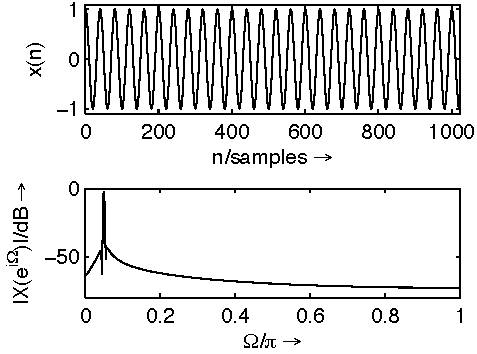
\includegraphics[scale=0.8]{fft_plot2}}
%\caption{{\it Sinusoid in time and frequency domain.}}  
%\label{fft_plot}
%\end{figure}
%Figures must be vectorial (no screen copy, no bitmap, etc). For example when using \texttt{Matlab}, export using either Postscript or PDF format. Also, in order to provide a better readibility, figure text font size should be at list identical to footnote font size. To do so using \texttt{Matlab}, use the \texttt{subplot} command before plotting.

%\subsection{Tables} 
%As for figures, all tables should be centered on the column (or page, if the table spans both columns). 
%Table captions should be in italic, follow each table and have the format given in Table \ref{tab:example}.

%\begin{table}[htdp]
%  \begin{center}
%    \begin{tabular}{|c|c|}\hline
%    	angle ($\theta$, rad) & $\sin \theta$ \\\hline
%	$\frac{\pi}{2}$ & 1 \\
%	$\pi$ & 0 \\
%	$\frac{3\pi}{2}$ & -1 \\
%	$2\pi$ & 0 \\\hline
%    \end{tabular}
%  \end{center}
%  \label{tab:example}
%  \caption{{\it Basic trigonometric values.}}
%\end{table}%

%\subsection{Equations}
%Equations should be placed on separate lines and numbered:

%\begin{equation}
%X(e^{j\Omega})=\sum_{n=0}^{N-1}x(n)e^{-j\Omega n}
%\label{eq1}
%\end{equation}
%where the sequence $x(n)$ in equation (\ref{eq1}) is a windowed frame:
%\begin{equation}
%x(n)=s(n)\cdot w(n)
%\label{eq2}
%\end{equation}
%with a window function $w(n)$.

%\subsection{Page Numbers}
%Page numbers will be added to the document electronically, so {\em please leave the numbering as is},
%that is, the first page will start at page DAFX-1 and the last page, at most, will have to be DAFX-6
%for the submission of papers for an oral presentation or DAFX-4 in the case of a poster presentation.

%\subsection{References}
%The references will be numbered in order of appearance \cite{Mitra:Kaiser:1993:DSP:handbook}, \cite{Haykin:1991:adaptive:filter}, \cite{Moorer:2000:AES:audio:millenium} and \cite{Arfib:1998:DAFx}. Please avoid listing references that do not appear in the text (we did the opposite in this template).

%\subsubsection{Reference Format}
%The reference format is the standard IEEE one. We recommend to use BibTeX to create the reference list.

%\section{Conclusions}
%This template can be found on the conference website. 
%If you wish to include two authors' affiliations please use the companion LaTeX template tmpl\_la2\_href. 
%Please, submit full-length papers (max.~6 pages for oral presentation and max.~4 pages for posters).
% 
%Submission is fully electronic and automated through the Conference Web Submission System. 
%DO NOT send us papers directly by e-mail. 

%\section{Acknowledgements}
%Many thanks to the great number of anonymous reviewers!

%%\newpage
%\nocite{*}
%\bibliographystyle{IEEEbib}
%\bibliography{template} % requires file template.bib

%\end{document}
